\documentclass{article}
\usepackage[spanish]{babel}
\usepackage[pdftex]{graphicx,color} 
\usepackage[utf8]{inputenc}
\usepackage{listings}
\usepackage{colortbl}
\usepackage{textcomp}
\usepackage{listings}
\usepackage{color}
\usepackage{wrapfig}
\usepackage{amsfonts}
\usepackage{amssymb}
\usepackage{algorithmic}
\usepackage{algorithm}
\usepackage[export]{adjustbox}
%\usepackage{amslatex}
\definecolor{lbcolor}{rgb}{0.9,0.9,0.9}
\lstset{
        backgroundcolor=, %\color{lbcolor},
        tabsize=4,
        rulecolor=,
        language=C,
        basicstyle=\scriptsize,
        upquote=true,
        aboveskip={1.5\baselineskip},
        %columns=fixed,
        showstringspaces=false,
        extendedchars=true,
        breaklines=true,
        prebreak = \raisebox{0ex}[0ex][0ex]{\ensuremath{\hookleftarrow}},
        frame=single,
        showtabs=false,
        showspaces=false,
        showstringspaces=false,
        identifierstyle=\ttfamily,
        keywordstyle=\color[rgb]{0,0,1},
        commentstyle=\color[rgb]{0.133,0.545,0.133},
        stringstyle=\color[rgb]{0.627,0.126,0.941},
	literate={á}{{\'a}}1
	{ã}{{\~a}}1
	{é}{{\'e}}1
	{ó}{{\'o}}1
	{í}{{\'i}}1
	{ñ}{{\~n}}1
	{¡}{{!`}}1
	{¿}{{?`}}1
	{ú}{{\'u}}1
	{Í}{{\'I}}1
	{Ó}{{\'O}}1
}

\topmargin -0.5in
\textwidth 6.8in
\textheight 9.0in
\oddsidemargin 0.0in
\evensidemargin 0.0in

\usepackage{enumitem}
\usepackage{multirow}
\usepackage{hhline}
\usepackage{multicol}
%ointpoints{punto}{puntos}

\begin{document}
\vspace{.5pc}
\centerline{\sc Clase Activa 5}
\centerline{\sc ELO320 - Estructura de Datos y Algoritmos}
\centerline{\sc Prof. Nicolás Gálvez Ramírez}
\vspace{2pc}
%\noindent {\bf Instrucciones}:
%\begin{itemize}
%    \item Conteste cada pregunta en una hoja separada. Éstas serán entregadas de tal forma al finalizar el certamen.
%    \item Si decide no contestar una pregunta, debe entregar una hoja sin respuestas en su lugar. 
%    \item Rotule claramente cada una de sus hojas con su Nombre Completo, Rol USM y Número de Paralelo.
%    \item El certamen tiene una duración de 60 minutos.
%\end{itemize}

%\noindent {\bf Preguntas}
%\medskip
\begin{itemize}

\begin{minipage}[h]{0.45\textwidth}
\item \textbf{Taxonomía de la memoria}. Rellene con su apunte a qué corresponde cada memoria y que tipo de elementos se almacenan en ellas.
\begin{enumerate}
\item text: 
\item static:
\item heap:
\item stack: 
\end{enumerate} 
\begin{center}
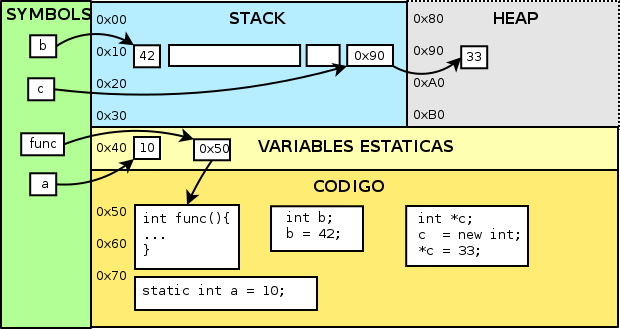
\includegraphics[width=.95\linewidth]{../images/progmemoria}
\end{center}
\end{minipage}
\hspace{0.5cm}
\begin{minipage}[h]{0.45\textwidth}
\item \textbf{malloc()}: Instrucción para la reserva de memoria que entrega como resultado la dirección de memoria donde inicia la reserva. \textbf{Necesitamos punteros}. Operador \texttt{sizeof} como base del tamaño a reservar. 
\begin{lstlisting}[language=C, basicstyle=\tiny, escapeinside={|}{|}]
#include<stdio.h>
#include<stdlib.h>

int main(int argc, char **argv){
	int *arreglo=NULL;
	arreglo = malloc(10 * sizeof(*arreglo));
//	arreglo = malloc(10 * sizeof(int));
//	arreglo = malloc(10 * sizeof *arreglo); 

// sizeof es un operador: sizeof(tipo_de_dato) o sizeof expresion
// cast no es necesario, compilador hace coerción.
// solo para compatibilidad con C++, se usa
//	arreglo = (int *) malloc(10 * sizeof(int)); 
	return 0;
}
\end{lstlisting}
\end{minipage}

\begin{minipage}[h]{0.45\textwidth}
\item \textbf{realloc()}: Instrucción para la reasignar memoria ya reservada. Si se agranda la memoria, esta puede cambiar completamente de dirección.
\begin{lstlisting}[language=C, basicstyle=\tiny, escapeinside={|}{|}]
#include<stdio.h>
#include<stdlib.h>

int main(int argc, char **argv){
	int *arreglo=NULL;

	arreglo = malloc(10 * sizeof(*arreglo));

	// libera 5 ints, mantiene dir.
	arreglo = realloc(arreglo, 5 * sizeof(int));

	// se expande en 15 ints, mantiene dir si existe
	// espacio contiguo, sino se cambia.
	arreglo= realloc(arreglo, 20 * sizeof * arreglo);

	return 0;
}
\end{lstlisting}
\end{minipage}
\hspace{0.5cm}
\begin{minipage}[h]{0.45\textwidth}
\item \textbf{free()}: Instrucción para liberar la memoria reservada en heap. Sirve para liberar los recursos ociosos y no acaparar recursos en el manejo (memory leaks). \textbf{Ejemplos anteriores no liberan memoria}.

\begin{lstlisting}[language=C, basicstyle=\tiny, escapeinside={|}{|}]
#include<stdio.h>
#include<stdlib.h>

int main(int argc, char **argv){
	int *arreglo=NULL;

	arreglo = malloc(10 * sizeof(*arreglo));

	// libera 5 ints, mantiene dir.
	arreglo = realloc(arreglo, 5 * sizeof(int));

	// se expande en 15 ints, mantiene dir si existe
	// espacio contiguo, sino se cambia.
	arreglo= realloc(arreglo, 20 * sizeof * arreglo);

	free(arreglo);
	return 0;
}
\end{lstlisting}
\end{minipage}

\begin{minipage}[h]{0.45\textwidth}
\item \textbf{Fuga de memoria (memory leak)}: Pérdida de acceso a objeto de memoria reservado en el heap, por no existir variables que apunten a él. No se puede liberar hasta el término del programa. Puede saturar la memoria.
\begin{lstlisting}[language=C, basicstyle=\tiny, escapeinside={|}{|}]
int main(int argc, char **argv){
	int *p;
	
	p= malloc(sizeof(int));
	p= malloc(sizeof(int));
	/* se pierde la direccion asignada anteriormente */

	free(p);

	return 0;
\end{lstlisting}

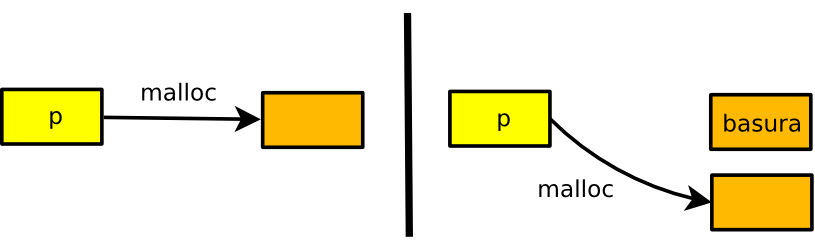
\includegraphics[width=.85\linewidth]{images/lostheap}\\


\end{minipage}
\hspace{0.5cm}
\begin{minipage}[h]{0.45\textwidth}
\item \textbf{Dejar Colgado (dangling)}: Puntero hacia localización de memoria del heap que ha sido liberada (e incluso nuevamente asignada). Genera errores poco predecibles (e.g. Segmentation fault, corrupción de memoria).
\begin{lstlisting}[language=C, basicstyle=\tiny, escapeinside={|}{|}]
int main(int argc, char **argv){
	int x=2;
	int *p, *q;

	p= malloc(sizeof(int));
	q=p;

	free(p);  /* q aun mantiene referencia al heap */
        	 /* puede que variable de heap sea reasignada */

	*q = x;

	return 0;
}
\end{lstlisting}
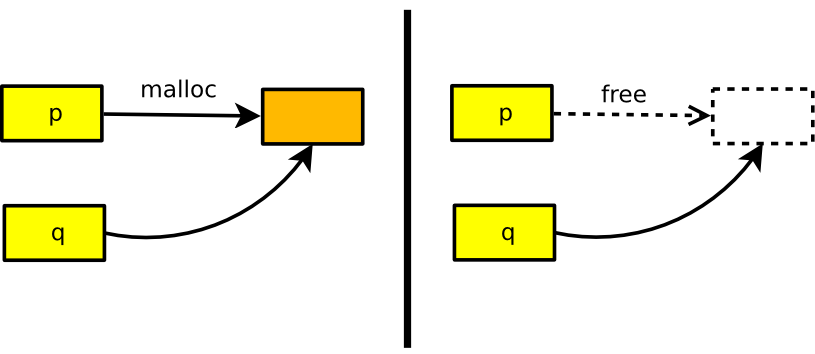
\includegraphics[width=.85\linewidth]{images/dangling}

\end{minipage}


\end{itemize}
\end{document}

